% !TEX root = ../OT4ML.tex

\chapter{Beyond Comparing Measures}
\label{sec-beyond-comparing-measures}

This chapter leaves the setting of scalar measures on a common ambient space. Vector- and matrix-valued OT transports mass with internal degrees of freedom, Gromov--Wasserstein compares metric-measure spaces without a prescribed correspondence, and quantum OT replaces scalar couplings by positive operators. In each case, the transport plan must also encode structure carried by the support, the fibers or the non-commutative state space.
\index{positive!operator}% strictindex
\index{plan!transport}% strictindex
\index{correspondence}% strictindex
\index{quantum!OT}% strictindex
\index{metric-measure space}% strictindex
\index{Gromov-Wasserstein@Gromov--Wasserstein}% strictindex
\index{Gromov-Wasserstein@Gromov--Wasserstein!distance}% strictindex

\section{Vector and Matrix-Valued Measures}
\index{vector-valued measure}% strictindex
\index{matrix-valued measure}% strictindex
\label{sec-vector-matrix-valued-measures}

Scalar OT transports a nonnegative density. In imaging, color processing, spectral analysis, diffusion tensor imaging and quantum-inspired models, the object attached to a point can instead have several nonnegative components or a positive semidefinite matrix. The first step beyond scalar OT is the positive vector-valued case: the fiber remains linear and commutative, but the transport cost may couple its channels.
\index{positive!semidefinite matrix}% strictindex

\paragraph{Positive vector-valued measures.}
\index{positive!vector-valued measure}% strictindex

The simplest way to keep internal structure in transport is to attach several nonnegative masses to each spatial point and to decide whether these channels move independently or interact through the cost.
\begin{defn}[Positive vector-valued measure]\label{def-positive-vector-valued-measure}
\index{vector-valued measure}% strictindex
	A positive $\RR_+^m$-valued measure on $\X$ is a tuple
	\[
		\al=(\al^1,\ldots,\al^m)\in\Mm_+(\X;\RR_+^m),
	\]
	where each component $\al^k$ is a nonnegative finite measure.
\end{defn}
This models multi-channel densities such as spectral bins or several species transported on the same domain. In a conservative model the mass of each channel is preserved, so one assumes $\al_0^k(\X)=\al_1^k(\X)$ for every $k$. The natural vector-valued extension of OT therefore starts from the positive cone $\RR_+^m$.
\index{finite measure}% strictindex
\index{positive!cone}% strictindex

For the dynamic formulas below, assume that $\X$ is either $\RR^d$, the flat torus, or a bounded convex domain in $\RR^d$ equipped with no-flux boundary conditions. First suppose that the endpoints and the curve have densities. The direct analogue of Benamou--Brenier fixes a vector density $u_t(x)\in\RR_+^m$ and a spatial flux
\index{flux}% strictindex
\index{Benamou-Brenier@Benamou--Brenier}% strictindex
$V_t(x)=(V_{t,1},\ldots,V_{t,d})\in(\RR^m)^d$, where $V_{t,\ell}^k$ is the velocity of channel $1\leq k\leq m$ in spatial direction $1\leq\ell\leq d$. The conservative vector transport cost associated with an action density $\Phi$ is
\index{velocity}% strictindex
\begin{equation}\label{eq-vector-valued-bb}
	\mathcal W_{\Phi}^2(\al_0,\al_1)
	\eqdef
	\inf_{u,V}
	\int_0^1\!\int_\X
	\Phi(u_t(x),V_t(x))\,\d x\,\d t
\end{equation}
subject to the endpoint constraints $u_0\d x=\al_0$, $u_1\d x=\al_1$ and the componentwise continuity equation
\index{continuity equation}% strictindex
\begin{equation}\label{eq-vector-valued-continuity}
	\partial_t u_t+\nabla_x\cdot V_t=0,
	\qquad
	(\nabla_x\cdot V_t)^k=\sum_{\ell=1}^d \partial_{x_\ell} V_{t,\ell}^k .
\end{equation}
Thus each component satisfies its own continuity equation, but the cost may still couple the components. Singular curves are handled as in scalar dynamic OT by replacing densities and fluxes by measures and using the lower semicontinuous perspective recession convention.
\index{perspective recession}% strictindex
\index{recession convention}% strictindex
\index{flux}% strictindex
\index{lower semicontinuity}% strictindex
\index{continuity equation}% strictindex

The notation $\mathcal W_\Phi$ does not by itself imply a distance for an arbitrary action $\Phi$. A sufficient set of structural conditions is reversibility $\Phi(u,-V)=\Phi(u,V)$ and quadratic time scaling $\Phi(u,sV)=s^2\Phi(u,V)$ for $s\geq0$, together with lower semicontinuity and coercive nondegeneracy, so that a sequence of curves with vanishing action cannot join two distinct endpoints. Time reversal then gives symmetry, while concatenation with an optimal allocation of time gives the triangle inequality for the square root of~\eqref{eq-vector-valued-bb}. Under these assumptions $\mathcal W_\Phi$ is an extended distance on each finite-action component. Componentwise conservation makes equality of all channel masses necessary for finiteness; without the preceding assumptions,~\eqref{eq-vector-valued-bb} is only a dynamic transport cost and may be asymmetric or degenerate.

The following elementary family separates independent channel motion from genuinely coupled vector transport.

\begin{example}[Diagonal and coupled positive mobilities]
Choose a mobility matrix $\mathsf M(u)\in\mathbb S_+^m$, where $\mathbb S_+^m$ denotes the cone of real symmetric positive semidefinite matrices, and set
\index{positive!semidefinite matrix}% strictindex
\[
	\Phi_{\mathsf M}(u,V)
	=
	\sum_{\ell=1}^d V_{\ell}^{\top}\mathsf M(u)^\dagger V_{\ell},
\]
with the usual convention that the value is finite only when each $V_\ell$ belongs to the range of $\mathsf M(u)$. If $u\mapsto\mathsf M(u)$ is linear and takes values in $\mathbb S_+^m$, then this action is jointly convex and positively one-homogeneous in $(u,V)$. Indeed, the matrix fractional map $(M,z)\mapsto z^\top M^\dagger z$ is jointly convex on its effective domain, and linearity gives $\mathsf M(su)=s\mathsf M(u)$ for $s>0$. For $m=1$ and $\mathsf M(u)=u$, one recovers exactly the scalar Benamou--Brenier action. For
\index{Benamou-Brenier@Benamou--Brenier}% strictindex
	\begin{equation}\label{eq-diagonal-vector-mobility}
		\mathsf M_{\mathrm{diag}}(u)=\diag(u_1,\ldots,u_m),
	\end{equation}
the channels move independently. Non-diagonal mobilities are the simplest way to couple the coordinates while keeping the same componentwise conservation law. For instance, with $q=m^{-1/2}(1,\ldots,1)$ and $\kappa\geq0$,
\[
	\mathsf M_\kappa(u)=\diag(u)+\kappa\Big(\sum_{k=1}^m u_k\Big) q q^\top
\]
increases the mobility in the common channel direction $q$ while leaving transverse directions controlled by the diagonal part. The local cost of moving one component can therefore depend on the densities and velocities of the other components, even though each component mass remains conserved.
\index{velocity}% strictindex
\end{example}

For the linear mobility actions $\Phi_{\mathsf M}$ above, these requirements hold: the action is even and quadratic in $V$, while the range convention and finite-dimensional coercivity make it separating on its effective domain. Their lower-semicontinuous measure extensions therefore define extended distances on the finite-action components with prescribed channel masses. In particular, writing $m_k=\al_0^k(\X)=\al_1^k(\X)$, the diagonal choice~\eqref{eq-diagonal-vector-mobility} gives the weighted product metric whose squared value is $\sum_{k:m_k>0}m_k\Wass_2^2(\al_0^k/m_k,\al_1^k/m_k)$.

The conservative positive-cone model above is the basic extension of Benamou--Brenier. Adding a source term $\partial_t u+\nabla\cdot V=S$ and a convex perspective penalty in $S$ gives unbalanced or reaction--transport variants. Such generalized transport models with dissipation and density modulation were developed by Maas, Rumpf, Sch{\"o}nlieb and Simon~\cite{maas2015generalized,maas2016generalized}; related nonlinear mobility distances and gradient structures appear in~\cite{dolbeault2009new,MielkeCVPDE}. Figure~\ref{fig:vector-valued-measure-geodesics} contrasts the exact diagonal case $\kappa=0$, where each positive channel is transported by its quantile map, with a large-$\kappa$ illustrative common-mode interpolation in which the channels move more coherently. The endpoints are two-mode mixtures: at each spatial mode the two channels have Gaussian profiles with the same center but different amplitudes.
\index{gradient!structure}% strictindex
\index{vector-valued measure}% strictindex
\index{positive!cone}% strictindex
\index{quantile!map}% strictindex

\begin{figure}[H]
\centering
\begin{tabular}{@{}cc@{}}
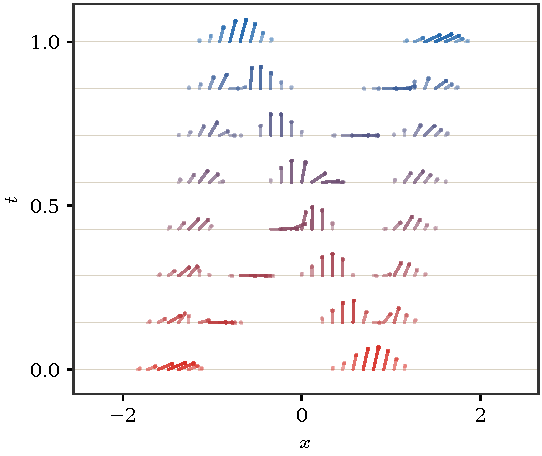
\includegraphics[width=.45\linewidth]{figures/vector-valued-measure-geodesics--kappa-zero-arrows.pdf} &
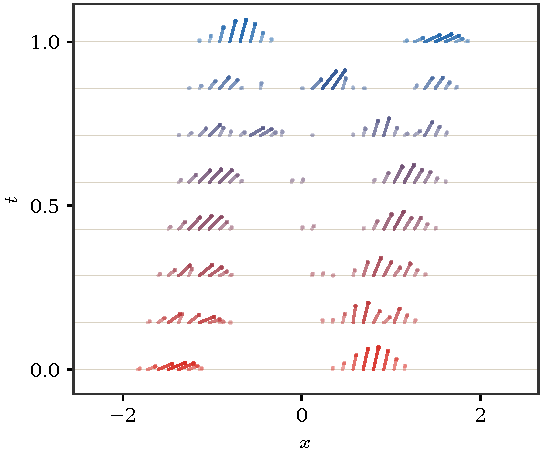
\includegraphics[width=.45\linewidth]{figures/vector-valued-measure-geodesics--kappa-large-arrows.pdf}
\\[-.1em]
\small independent channels $(\kappa=0)$ &
\small strongly coupled channels $(\kappa\gg1)$
\end{tabular}
\caption{\emph{One-dimensional positive $\RR_+^2$-valued transport displayed by arrow glyphs at eight time levels.} Each endpoint is a mixture of two localized Gaussian modes, and, inside each mode, both channel profiles have the same center. Each arrow is proportional to the local fiber value $(u_t^1(x),u_t^2(x))$, and time runs vertically from the red source to the blue target. Left: for $\kappa=0$, the diagonal mobility~\eqref{eq-diagonal-vector-mobility} gives two independent scalar quantile geodesics. Right: a large-$\kappa$ common-mode interpolation bends the display toward the direction $q=2^{-1/2}(1,1)$, illustrating the qualitative effect of a mobility that favors coherent channel motion while keeping the same componentwise continuity equation.}
\index{continuity equation}% strictindex
\label{fig:vector-valued-measure-geodesics}
\end{figure}

\paragraph{Positive matrix-valued measures.}
\index{matrix-valued measure}% strictindex
\index{positive!matrix-valued measure}% strictindex
The next simplest fiber is the positive matrix cone. This is the simplest tensor-valued model beyond vectors: the diagonal entries behave like positive channels, while the eigenvectors encode local orientations.

\begin{defn}[Positive matrix-valued measure]\label{def-positive-matrix-valued-measure}
\index{matrix!cone}% strictindex
	Write $\mathbb S^m$ for real symmetric matrices and $\mathbb S_+^m$ for the positive semidefinite cone. A positive $\mathbb S_+^m$-valued measure is a countably additive map from Borel sets of $\X$ to $\mathbb S_+^m$; we denote the cone of such measures by
	\[
		\mathcal A\in\Mm_+(\X;\mathbb S_+^m).
	\]
\end{defn}
Equivalently, $\mathcal A$ is a symmetric matrix of finite signed measures such that $\mathcal A(E)\succeq0$ for every Borel set $E$. If $\mathcal A$ has density $A(x)\succeq0$, then $\tr A(x)$ is the scalar amount of mass at $x$, while, wherever $\tr A(x)>0$, the normalized matrix $A(x)/\tr A(x)$ records an internal covariance or orientation. This is the matrix analogue of the positive vector case: diagonal matrices encode nonnegative vector components, and non-diagonal matrices add a local eigenbasis.

The conservative Benamou--Brenier model fixes a matrix density $A_t(x)\in\mathbb S_+^m$ and symmetric matrix fluxes $P_t(x)=(P_{t,1},\ldots,P_{t,d})\in(\mathbb S^m)^d$. With no flux through the boundary of $\X$, the full matrix mass $\int_\X A_t(x)\d x$ is conserved, so the endpoints must have the same total matrix. The model minimizes the matrix-perspective action
\index{flux}% strictindex
\index{Benamou-Brenier@Benamou--Brenier}% strictindex
\begin{equation}\label{eq-matrix-valued-bb}
\begin{aligned}
\mathcal W_{\mathrm{mat}}^2(\mathcal A_0,\mathcal A_1)
\eqdef
\inf_{A,P}\int_0^1\!\int_\X
\sum_{\ell=1}^d \tr\big(P_{t,\ell}^{\top} A_t^\dagger P_{t,\ell}\big)\d x\d t
\end{aligned}
\end{equation}
subject to $A_0\d x=\mathcal A_0$, $A_1\d x=\mathcal A_1$ and to the matrix-valued continuity equation
\index{matrix-valued measure}% strictindex
\index{continuity equation}% strictindex
\begin{equation}\label{eq-matrix-valued-continuity}
\partial_t A_t+\nabla_x\cdot P_t=0,
\qquad
\nabla_x\cdot P_t=\sum_{\ell=1}^d \partial_{x_\ell}P_{t,\ell}.
\end{equation}
Here $A^\dagger$ denotes the Moore--Penrose inverse, with the usual lower-semicontinuous perspective convention: the action is finite only when the columns of each $P_{t,\ell}$ belong to the range of $A_t$. The matrix fractional map $(A,P)\mapsto\tr(P^{\top}A^\dagger P)$ is jointly convex on this effective domain and positively one-homogeneous in $(A,P)$. This gives the simplest non-trivial matrix-valued transport model: spatial motion is conservative, but the fiber carries orientation through the eigenvectors of $A_t(x)$.

Here $\mathcal W_{\mathrm{mat}}$ is an extended distance. Indeed, the action is invariant under $P\mapsto-P$, quadratic under time rescaling and zero only for $P=0$ on its effective domain. These facts give symmetry, the triangle inequality and definiteness, respectively. It is finite only between endpoints joined by a finite-action curve; equality of their total matrices is necessary but need not by itself guarantee finiteness. Thus $\mathcal W_{\mathrm{mat}}$ is a genuine distance on each finite-action component and takes the value $+\infty$ between distinct components.

\begin{prop}[Diagonal matrix subproblem]\label{prop-matrix-diagonal-reduction}
\index{matrix!subproblem}% strictindex
Assume that the endpoints are diagonal in a fixed orthonormal basis,
\[
	\mathcal A_i=\diag(\al_i^1,\ldots,\al_i^m),
	\qquad i=0,1,
\]
and that $\al_0^k(\X)=\al_1^k(\X)=m_k$ for every $k$. If one restricts the admissible curves in~\eqref{eq-matrix-valued-bb} to remain diagonal in that basis,
\[
	A_t=\diag(u_t^1,\ldots,u_t^m),
	\qquad
	P_{t,\ell}=\diag(V_{t,\ell}^1,\ldots,V_{t,\ell}^m),
\]
then the value of this restricted matrix problem is
\[
	\sum_{k:m_k>0} m_k\,\Wass_2^2\!\left(\frac{\al_0^k}{m_k},\frac{\al_1^k}{m_k}\right),
\]
with zero contribution from zero-mass channels. Thus the commuting matrix submodel is exactly the positive vector-valued Benamou--Brenier model associated with the diagonal mobility~\eqref{eq-diagonal-vector-mobility}.
\index{Benamou-Brenier@Benamou--Brenier}% strictindex
\end{prop}
\begin{proof}
The continuity equation~\eqref{eq-matrix-valued-continuity} is diagonal entry by diagonal entry and gives $\partial_t u^k+\nabla\cdot V^k=0$. Moreover,
\index{continuity equation}% strictindex
\[
	\sum_{\ell=1}^d \tr\big(P_{t,\ell}^{\top}A_t^\dagger P_{t,\ell}\big)
	=
	\sum_{k=1}^m \frac{|V_t^k|^2}{u_t^k}
\]
with the same scalar perspective convention as before. The admissible set and the action are therefore exactly those of the diagonal vector model.
\end{proof}

The restriction to a fixed diagonal basis gives eigenvalue transport; it should be read as a commuting submodel, not as a claim that non-diagonal excursions can never change the unrestricted value. The genuinely matrix-valued case starts when the eigenspaces vary with $x$ or along the interpolation, so that the transported object carries both mass and orientation. Static matrix-valued Monge--Kantorovich problems and dual test-function metrics were developed in~\cite{Ning2014metrics,JiangSpectral,ning2015matrix}; dynamic versions and related non-commutative geometries appear in~\cite{Chen2016,ChenGangbo17,Carlen2014,2016-peyre-qot}. Figure~\ref{fig:matrix-valued-measure-geodesic} shows the analogous independent/coupled contrast for positive $2\times2$ matrix fibers, using two localized matrix modes whose eigenvalue profiles share a common center at each mode.
\index{Kantorovich!problem}% strictindex
\index{matrix-valued measure}% strictindex

\begin{figure}[H]
\centering
\begin{tabular}{@{}cc@{}}
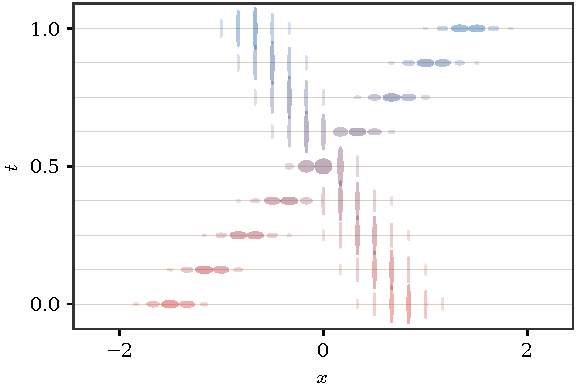
\includegraphics[width=.46\linewidth]{figures/matrix-valued-measure-geodesic--independent-ellipses.pdf} &
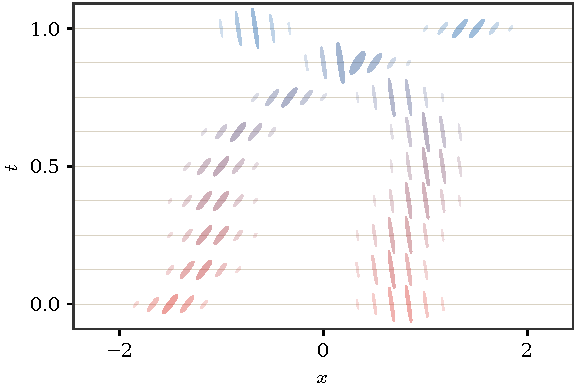
\includegraphics[width=.46\linewidth]{figures/matrix-valued-measure-geodesic--coupled-ellipses.pdf}
\\[-.1em]
\small commuting tensor channels &
\small strongly coupled tensor fibers
\end{tabular}
\caption{\emph{Positive $2\times2$ matrix-valued transport on a one-dimensional base.} Each endpoint is a mixture of two localized matrix modes; within one mode, both eigenvalue profiles are Gaussian bumps with the same center. Each ellipse is the glyph of a positive semidefinite matrix $A_t(x)$, with axes given by eigenvectors and eigenvalues. Left: the matrices are diagonal in a fixed basis, giving the commuting tensor analogue of independent vector channels. Right: a coupled illustrative interpolation bends packet motion toward the trace-density transport and uses non-commuting eigendirections; the superposition remains positive semidefinite and produces spatially varying orientations.}
\index{positive!semidefinite matrix}% strictindex
\label{fig:matrix-valued-measure-geodesic}
\end{figure}


\section{Wasserstein over Wasserstein}
\index{Wasserstein!over Wasserstein}% strictindex
\label{sec-wasserstein-over-wasserstein}

The Wasserstein construction can itself be iterated: once $(\X,\dist)$ is a metric space, $(\Pp_p(\X),\Wass_p)$ is again a metric space and can serve as the ground space for another Wasserstein distance. This is useful when the objects to compare are random probability measures, or mixtures whose components are meaningful objects rather than only a collapsed density. We first record the structure of this new ground space, then distinguish a law of measures from its collapsed mixture, and finally transport such laws.
\index{probability measure}% strictindex
\index{random probability measure}% strictindex

\paragraph{Wasserstein spaces as ground spaces.}
The standard setting is that of Polish spaces, introduced in Definition~\ref{def-polish-metric-space}. These assumptions rule out many measure-theoretic pathologies: probability laws can be approximated by countable objects, tightness gives compactness criteria, regular conditional probabilities exist on the associated Borel spaces, and weak convergence is stable. The next proposition records that Wasserstein spaces preserve this structure, so the construction can be iterated without leaving the same well-behaved category.
\index{conditional!probability}% strictindex
\index{tightness}% strictindex
\index{Wasserstein!space}% strictindex
\index{weak!convergence}% strictindex
\index{Polish space}% strictindex

\begin{prop}[Wasserstein spaces as ground spaces]\label{prop-wasserstein-space-polish}
	Let $1\leq p<\infty$. If $(\X,\dist)$ is Polish, then $(\Pp_p(\X),\Wass_p)$ is Polish. If $\X$ is compact, then $\Pp_p(\X)=\Pp(\X)$ and this space is compact for $\Wass_p$. Consequently, one may iterate the construction, with the corresponding finite-moment condition at every level.
\index{Wasserstein!topology}% strictindex
\end{prop}
\begin{proof}
	This is a standard structural theorem for Wasserstein spaces~\cite{Villani09,SantambrogioBook,ambrosio2006gradient}. For completeness, extract from a $\Wass_p$-Cauchy sequence a subsequence $(\alpha_k)_k$ such that $\sum_k\Wass_p(\alpha_k,\alpha_{k+1})<\infty$. Gluing optimal couplings of consecutive terms produces random variables $(X_k)_k$ with laws $\alpha_k$ and $\sum_k\norm{\dist(X_k,X_{k+1})}_{L^p}<\infty$. Hence $X_k$ converges almost surely and in $L^p$ to an $\X$-valued random variable; its law is the $\Wass_p$ limit of the subsequence, and the Cauchy property gives convergence of the original sequence. Separability follows by approximating measures with finitely supported measures on a countable dense subset and rational weights. If $\X$ is compact, Prokhorov's theorem gives compactness of $\Pp(\X)$ for weak convergence, and Proposition~\ref{prop-wass-metrizes-weak-compact} identifies this topology with the $\Wass_p$ topology.
\index{countable dense subset}% strictindex
\index{Wasserstein!space}% strictindex
\index{rational weights}% strictindex
\index{weak!convergence}% strictindex
\end{proof}

\paragraph{Random measures and collapsed mixtures.}
Fix $1\leq p<\infty$. We denote elements of $\Pp_p(\X)$ by $\alpha,\beta,\ldots$. Elements of $\Pp_p(\Pp_p(\X))$ are denoted by fraktur letters, for instance $\mathfrak A,\mathfrak B$; they are probability laws over probability measures, or random probability measures. A basic parametric example is obtained from a measurable family $(\alpha_\zeta)_{\zeta\in Z}$ and a probability law $\gamma$ on the parameter space:
\index{probability measure}% strictindex
\index{random probability measure}% strictindex
\begin{equation}\label{eq-wow-parametric-law}
	\mathfrak A=(\zeta\mapsto\alpha_\zeta)_\sharp\gamma.
\end{equation}
It belongs to $\Pp_p(\Pp_p(\X))$ precisely when, for one and hence every $x_0\in\X$,
\[
	\int_Z \Wass_p(\alpha_\zeta,\delta_{x_0})^p\,\d\gamma(\zeta)<\infty.
\]
If $\gamma=\sum_{i=1}^K a_i\delta_{\zeta_i}$, then
\[
	\mathfrak A=\sum_{i=1}^K a_i\delta_{\alpha_{\zeta_i}}.
\]
\begin{defn}[Collapsed, or barycentric, mixture]\label{def-collapsed-barycentric-mixture}
\index{collapsed mixture}% strictindex
\index{barycentric!mixture}% strictindex
	For $\mathfrak A\in\Pp(\Pp(\X))$, the collapsed, or barycentric, mixture associated with $\mathfrak A$ is the measure $\bar\alpha_{\mathfrak A}$ defined by
	\begin{equation}\label{eq-wow-barycentric-mixture}
		\int_\X f(x)\d\bar\alpha_{\mathfrak A}(x)
		=
		\int_{\Pp(\X)}
		\left(\int_\X f(x)\d\alpha(x)\right)
		\d\mathfrak A(\alpha),
	\end{equation}
	for bounded continuous $f$.
\end{defn}
The term ``barycentric mixture'' should not be confused with the Wasserstein barycenter defined by~\eqref{eq-barycenter-generic} in Section~\ref{sec-barycenters}. The collapse~\eqref{eq-wow-barycentric-mixture} is linear in $\mathfrak A$, whereas a Wasserstein barycenter gives a nonlinear way to reduce a law over measures to one measure by minimizing its average transport cost.
In the finite case, $\bar\alpha_{\mathfrak A}=\sum_i a_i\alpha_{\zeta_i}$. Moreover, if $\mathfrak A\in\Pp_p(\Pp_p(\X))$, then $\bar\alpha_{\mathfrak A}\in\Pp_p(\X)$ because
\[
	\int_\X \dist(x,x_0)^p\,\d\bar\alpha_{\mathfrak A}(x)
	=
	\int_{\Pp_p(\X)}\Wass_p(\alpha,\delta_{x_0})^p\,\d\mathfrak A(\alpha).
\]

\paragraph{Transport between random measures.}
Having equipped $\Pp_p(\X)$ with the ground distance $\Wass_p$, one applies the ordinary Kantorovich construction to probability laws on this space:
\index{Wasserstein!distance}% strictindex
\index{Wasserstein!space}% strictindex
\begin{equation}\label{eq-wow-distance}
	\mathbb W_p^p(\mathfrak A,\mathfrak B)
	\eqdef
	\inf_{\Pi\in\Couplings(\mathfrak A,\mathfrak B)}
	\int_{\Pp_p(\X)\times\Pp_p(\X)}
	\Wass_p^p(\alpha,\beta)\d\Pi(\alpha,\beta),
	\qquad
	\mathfrak A,\mathfrak B\in\Pp_p(\Pp_p(\X)).
\end{equation}
For $p=2$, Gaussian mixtures provide a particularly explicit example with two levels of geometry. A mixture
\index{Gaussian!mixture}% strictindex
$\sum_i a_i\Gaussian(m_i,\Sigma_i)$ can either be viewed as the collapsed measure on $\X$, or as the component law
\[
	\mathfrak A=\sum_i a_i\delta_{\Gaussian(m_i,\Sigma_i)}
\]
on the Bures-Wasserstein space of Gaussian components. Given two component laws
\[
	\mathfrak A=\sum_i a_i\delta_{\Gaussian(m_i,\Sigma_i)},
	\qquad
	\mathfrak B=\sum_j b_j\delta_{\Gaussian(n_j,\Lambda_j)},
\]
the discrete problem induced by~\eqref{eq-wow-distance} uses the component cost
\[
	\C_{ij}=\norm{m_i-n_j}^2+\Bb(\Sigma_i,\Lambda_j)^2.
\]
Let $\P^\star$ be an optimal coupling between the weights $a$ and $b$. If $A_{ij}$ denotes the Brenier linear part from $\Sigma_i$ to $\Lambda_j$, then each active component pair is interpolated by
\[
	m_{ij,t}=(1-t)m_i+t n_j,
	\qquad
	\Sigma_{ij,t}
	=
	\big((1-t)\Id+tA_{ij}\big)\Sigma_i
	\big((1-t)\Id+tA_{ij}\big)^\top,
\]
and collapsing these component geodesics gives
\[
	\bar\alpha_t=
	\sum_{i,j}\P^\star_{ij}\Gaussian(m_{ij,t},\Sigma_{ij,t}).
\]
This component-level interpolation transports Gaussian components as atoms of the Wasserstein space before returning to measures on~$\X$. It is generally not the same as the true $\Wass_2$ interpolation between the collapsed mixture densities, which can split and recombine mass inside and across components.
\index{Bures!Wasserstein geometry}% strictindex
\index{collapsed mixture}% strictindex
\index{Wasserstein!space}% strictindex

Figure~\ref{fig:kantorovich-wow-mixtures} contrasts this component-level geodesic with the true one-dimensional Wasserstein interpolation of the collapsed mixtures, making the internal mass splitting absent from the former visible.

\begin{figure}[htbp]
\centering
\begin{tabular}{cc}
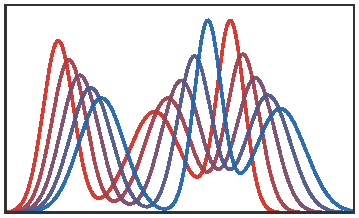
\includegraphics[width=.46\linewidth]{figures/kantorovich-wow-mixtures--component-level.pdf} &
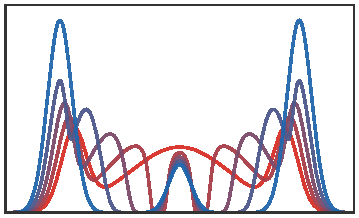
\includegraphics[width=.46\linewidth]{figures/kantorovich-wow-mixtures--collapsed-w2.pdf} \\[-.1em]
\small component law on Gaussian atoms &
\small collapsed mixture law
\index{collapsed mixture}% strictindex
\end{tabular}
\caption{\emph{Two interpolations between the same asymmetric three-component one-dimensional Gaussian mixtures.} The red endpoint has a broad central component carrying most of the mass, while the blue endpoint has two dominant sharp side modes. Left: Gaussian components are transported as atoms using their Bures-Wasserstein distance. Right: the collapsed densities are interpolated by the true one-dimensional quantile formula for $\Wass_2$. The central mass is split and recombined in the collapsed geometry, making the two paths visibly distinct.}
\index{Gaussian!mixture}% strictindex
\index{Wasserstein!distance}% strictindex
\index{quantile!formula}% strictindex
\label{fig:kantorovich-wow-mixtures}
\end{figure}

\begin{prop}[Collapsing is non-expansive]\label{prop-wow-collapsed-bound}
	Let $(\X,\dist)$ be Polish, let $1\leq p<\infty$, and let $\mathfrak A,\mathfrak B\in\Pp_p(\Pp_p(\X))$. For the collapsed mixtures defined by~\eqref{eq-wow-barycentric-mixture},
\index{barycentric!mixture}% strictindex
\index{collapsed mixture}% strictindex
	\[
		\Wass_p(\bar\alpha_{\mathfrak A},\bar\beta_{\mathfrak B})
		\leq
		\mathbb W_p(\mathfrak A,\mathfrak B).
	\]
\end{prop}
\begin{proof}
	Fix $\Pi\in\Couplings(\mathfrak A,\mathfrak B)$ and $\eta>0$. A standard measurable-selection theorem for optimal transport on Polish spaces gives a measurable kernel $(\alpha,\beta)\mapsto\pi_{\alpha,\beta}\in\Couplings(\alpha,\beta)$ such that
	\[
		\int_{\X\times\X}\dist(x,y)^p\,\d\pi_{\alpha,\beta}(x,y)
		\leq \Wass_p(\alpha,\beta)^p+\eta.
	\]
	Integrating this kernel against $\Pi$ gives a coupling $\bar\pi$ between $\bar\alpha_{\mathfrak A}$ and $\bar\beta_{\mathfrak B}$. Its cost satisfies
\index{measurable selection}% strictindex
\index{Markov kernel}% strictindex
\index{transport!cost}% strictindex
	\[
		\int_{\X\times\X}\dist(x,y)^p\d\bar\pi(x,y)
		\leq
		\int_{\Pp_p(\X)^2}\Wass_p^p(\alpha,\beta)\d\Pi(\alpha,\beta)+\eta.
	\]
	Letting $\eta\downarrow0$, taking the infimum over $\Pi$, and then taking the $p$-th root proves the claim.
\end{proof}

The following remark records a useful way in which this iterated construction reappears in the Gromov--Wasserstein lower bounds of the next section.

\begin{rem}[Local profiles as Wasserstein-over-Wasserstein laws]
	Given a metric-measure space $\XX=(\X,\dist_\X,\al_\X)$, each point defines a local distance distribution
\index{Wasserstein!distance}% strictindex
\index{Gromov-Wasserstein@Gromov--Wasserstein}% strictindex
\index{Gromov-Wasserstein@Gromov--Wasserstein!distance}% strictindex
\index{local distance distribution}% strictindex
\index{metric-measure space}% strictindex
\[
	\alpha_x=(\dist_\X(x,\cdot))_\sharp\al_\X\in\Pp(\RR_+),
	\qquad
	\mathfrak D_\XX=(x\mapsto\alpha_x)_\sharp\al_\X\in\Pp(\Pp(\RR_+)).
\]
The M\'emoli profile lower bound in Proposition~\ref{prop-memoli-gw-profile-lower-bound} is precisely a Wasserstein-over-Wasserstein comparison of these laws of local profiles. It replaces the full pairwise distortion by an ordinary OT problem whose ground cost is itself a one-dimensional Wasserstein distance.
\index{profile lower bound}% strictindex
\index{local profile}% strictindex
\index{distortion}% strictindex
\index{ground cost}% strictindex
\index{Memoli profile@M\'emoli profile}% strictindex
\index{Wasserstein!over Wasserstein}% strictindex
\index{Wasserstein!distance}% strictindex
%
\end{rem}

\section{Gromov--Wasserstein}
\index{Gromov-Wasserstein@Gromov--Wasserstein}% strictindex
\index{Gromov-Wasserstein@Gromov--Wasserstein!distance}% strictindex
\label{sec-gromov-wasserstein}

Gromov--Wasserstein compares spaces through their internal distance structures rather than through a fixed ambient ground cost. This is the right extension for graphs, shapes and point clouds whose points are not pre-aligned.
\index{ground cost}% strictindex

\paragraph{Discrete formulation.}

Optimal transport needs a ground cost $\C$ to compare histograms $(\a,\b)$, and thus cannot be used directly if the histograms are not defined on the same underlying space, or if one cannot pre-register these spaces to define a ground cost.
\index{histogram}% strictindex
%
To address this issue, one can instead use a weaker requirement: two matrices $\distD \in \RR^{n \times n}$ and $\distD' \in \RR^{m \times m}$ are available and represent relationships between the points on which the histograms are defined. A typical scenario is when these matrices are powers of distance matrices.
%
Define the quadratic distortion energy
\index{Gromov-Wasserstein@Gromov--Wasserstein}% strictindex
\begin{equation}\label{eq-gw-def}
\begin{aligned}
	\Ee_{\distD,\distD'}(\P)
	&\eqdef
	\sum_{i,j,i',j'} \De(\distD_{i,i'},\distD'_{j,j'})^p \P_{i,j}\P_{i',j'},
	\\
	\GWD( (\a,\distD), (\b,\distD') )^p
	&\eqdef
	\min_{\P \in \CouplingsD(\a,\b) }
	\Ee_{\distD,\distD'}(\P),
\end{aligned}
\end{equation}
where $p \geq 1$ and $\De$ is a distance on $\RR$, typically $\De(u,v)=|u-v|$.
%
This is a non-convex quadratic problem over the transport polytope. In the uniform case with the additional hard-assignment constraint $m=n$ and $\P$ a permutation matrix, it becomes a Quadratic Assignment Problem (QAP)~\cite{loiola-2007}; this restricted graph-matching form is already NP-hard in full generality.
\index{assignment problem}% strictindex
\index{quadratic!assignment problem}% strictindex
\index{matrix!permutation}% strictindex
\index{transportation polytope}% strictindex
%
The relaxed coupling formulation used in GW can therefore be read as a soft graph-matching model~\cite{lyzinski-2015}.

\begin{example}[Application to structured objects]\label{ex-structured-objects-gw}
\index{structured data}% strictindex
\index{graph!matching}% strictindex
	Graphs, molecules, meshes and point clouds often do not come with a common coordinate system or a reliable node-to-node correspondence. GW compares them through their internal distances, so the coupling \(\P_{ij}\) becomes a soft structural correspondence rather than a spatial displacement. This is useful for graph matching, node embedding, shape comparison and molecule or mesh alignment~\cite{peyre2016gromov,vayer2019optimaltransportstructured}. When node attributes are also available, fused GW below adds a feature transport term to the intrinsic distortion, separating what should be preserved as structure from what should be matched as signal.
\end{example}

Figure~\ref{fig:gromov-isometry-matching} shows this intrinsic matching principle under progressively stronger deformations: correspondences are selected from within-space distance patterns rather than an ambient cross-space cost.

\begin{figure}[ht]
\centering
\begin{tabular}{@{}ccc@{}}
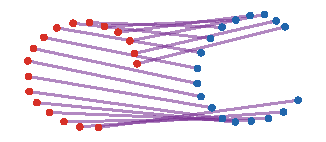
\includegraphics[width=.30\linewidth]{figures/gromov-isometry-matching--isometric.pdf} &
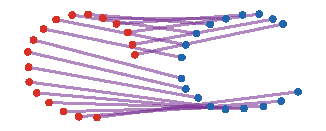
\includegraphics[width=.30\linewidth]{figures/gromov-isometry-matching--mild-deformation.pdf} &
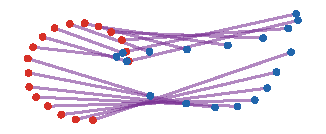
\includegraphics[width=.30\linewidth]{figures/gromov-isometry-matching--strong-deformation.pdf}
\\[-.1em]
\small isometric copy &
\small mild deformation &
\small strong deformation
\end{tabular}
\caption{\emph{Gromov--Wasserstein correspondences under increasing deformation.} The red and blue point clouds are not compared through an ambient Euclidean cross-cost; instead, the GW coupling compares their internal pairwise distances. A perfectly isometric copy admits a clean structural match, while mild and deliberately stronger deformations progressively bend the correspondence.}
\index{pairwise distance}% strictindex
\index{Gromov-Wasserstein@Gromov--Wasserstein}% strictindex
\index{correspondence}% strictindex
\label{fig:gromov-isometry-matching}
\end{figure}

When the matrices $\distD,\distD'$ are genuine distance matrices, the general construction below shows that $\GWD$ satisfies the triangle inequality and defines a distance between metric spaces equipped with a probability distribution, up to measure-preserving isometries.
\index{triangle inequality}% strictindex
\index{measure-preserving!isometry}% strictindex
%
This distance was introduced and studied in detail by Memoli in~\cite{memoli-2011}. An in-depth mathematical exposition (in particular, its geodesic structure and gradient flows) is given in~\cite{SturmGW}. See also~\cite{schmitzer2013modelling} for applications in computer vision.
\index{gradient!flow}% strictindex
%
Its relation to Hausdorff and Gromov--Hausdorff distances is discussed at the end of this section.
\index{Hausdorff distance}% strictindex
\index{Gromov-Hausdorff distance}% strictindex

%%%%%%%%%%%%%%%%%%%%%
\paragraph{General setting.}

The continuous formulation abstracts the discrete distance matrices into metric-measure spaces, so that GW compares intrinsic geometries independently of labels, parametrizations or ambient coordinates.
\begin{defn}[Metric-measure space]\label{def-metric-measure-space}
\index{metric-measure space}% strictindex
	A metric-measure space is a triple
	\[
		\XX=(\X,\dist_\X,\al),
	\]
	where $(\X,\dist_\X)$ is Polish and $\al$ is a Borel probability measure on $\X$. For a finite $p$-Gromov--Wasserstein distance, one additionally assumes the finite-size condition
	\[
		\int_{\X\times\X}\dist_\X(x,x')^p\,\d\al(x)\d\al(x')<\infty.
	\]
\end{defn}
The general setting corresponds to computing couplings between metric-measure spaces $\XX=(\X,\dist_\X,\al)$ and $\YY=(\Y,\dist_\Y,\be)$, where the distance and the measure are both part of the data. Compactness is often assumed below to avoid additional tightness and integrability arguments.
%
One defines
	\begin{align}
		\label{eq-gw-generic}
		\GW( \XX,\YY )^p \eqdef
		\umin{ \pi \in \Couplings(\al,\be) }
		\int_{\X^2 \times \Y^2}
		 \De(\dist_\X(x,x'),\dist_\Y(y,y'))^p
		\d\pi(x,y)\d\pi(x',y').
	\end{align}

\begin{prop}[Fixed-space GW is controlled by Wasserstein]\label{prop-gw-controlled-by-wasserstein}
	Let $\alpha,\beta\in\Pp_p(\X)$ be probability measures on the same metric space $(\X,\dist_\X)$, and take $\De(u,v)=|u-v|$ in~\eqref{eq-gw-generic}. Then
\index{probability measure}% strictindex
	\[
		\GW((\X,\dist_\X,\alpha),(\X,\dist_\X,\beta))
		\leq
		2\Wass_p(\alpha,\beta).
	\]
	The Wasserstein distance on the right is computed with the same ground metric $\dist_\X$. The factor $2$ comes from the normalization in~\eqref{eq-gw-generic}; with the alternative convention $\De(u,v)=|u-v|/2$, the displayed constant becomes $1$.
\index{Gromov-Wasserstein@Gromov--Wasserstein}% strictindex
\index{Wasserstein!distance}% strictindex
\end{prop}
\begin{proof}
	Let $\pi$ be any coupling between $\alpha$ and $\beta$. For two independent pairs $(X,Y),(X',Y')\sim\pi$, the reverse triangle inequality gives
\index{triangle inequality}% strictindex
	\[
		\big|\dist_\X(X,X')-\dist_\X(Y,Y')\big|
		\leq
		\dist_\X(X,Y)+\dist_\X(X',Y').
	\]
	Taking the $L^p$ norm and using Minkowski gives a bound by $2(\int\dist_\X(x,y)^p\d\pi)^{1/p}$. Optimizing over $\pi$ proves the claim.
\index{Minkowski inequality}% strictindex
\end{proof}

To turn GW from a distortion score into a metric statement, one must quotient out the relabelings that preserve both distances and mass.

\begin{defn}[Isometric metric-measure spaces]\label{def-isometric-mm-spaces}
\index{metric-measure space}% strictindex
\index{measure-preserving!isometry}% strictindex
	Two metric-measure spaces $\XX=(\X,\dist_\X,\al)$ and $\YY=(\Y,\dist_\Y,\be)$ are isometric if there exists a bijection $\phi:\supp(\al)\to\supp(\be)$ such that $\phi_\sharp\al=\be$ and
	\[
		\dist_\Y(\phi(x),\phi(x'))=\dist_\X(x,x')
	\]
	for all $x,x'\in\supp(\al)$.
\end{defn}

The next theorem explains why the averaged distortion above is not merely a matching score. Once one quotients out measure-preserving isometries, it defines a genuine distance between metric-measure spaces.
\index{distortion}% strictindex
\index{measure-preserving!isometry}% strictindex
\index{metric-measure space}% strictindex

\begin{thm}[Gromov--Wasserstein metric modulo isometries]\label{thm-gw-metric}
\index{Gromov-Wasserstein@Gromov--Wasserstein}% strictindex
\index{Gromov-Wasserstein@Gromov--Wasserstein!metric}% strictindex
\index{modulo isometry}% strictindex
	For compact metric-measure spaces, $p\geq1$ and $\De(u,v)=|u-v|$, $\GW$ defines a distance up to measure-preserving isometries.
\end{thm}

\begin{proof}
	Compactness of the supports makes the coupling set compact and the distortion functional continuous, so an optimal coupling exists. If $\phi$ is a measure-preserving isometry, the graph coupling $(\Id,\phi)_\sharp\al$ has zero distortion; in particular, $\GW(\XX,\XX)=0$. Symmetry and non-negativity are immediate.

	If $\GW(\XX,\YY)=0$ and $\pi$ is an optimal plan, then $\dist_\X(x,x')=\dist_\Y(y,y')$ holds $\pi\otimes\pi$-almost everywhere. By continuity, this equality holds on $\supp(\pi)^2$. We show that $\XX$ and $\YY$ are isometric by showing that both are isometric to the support space $(\supp(\pi),\dist_\pi,\pi)$, where
\index{optimal plan}% strictindex
	\[
		\dist_\pi((x,y),(x',y'))
		\eqdef
		\frac12\dist_\X(x,x')+\frac12\dist_\Y(y,y').
	\]
	The first projection $\psi:(x,y)\mapsto x$ is measure-preserving. For $((x,y),(x',y'))\in\supp(\pi)^2$,
	\[
		\dist_\X(\psi(x,y),\psi(x',y'))
		=
		\dist_\X(x,x')
		=
		\dist_\Y(y,y')
		=
		\dist_\pi((x,y),(x',y')),
	\]
	so $\psi$ is an isometry and therefore injective. To see surjectivity onto $\supp(\al)$, take $x\in\supp(\al)$. Since $\psi_\sharp\pi=\al$, there is a sequence $(x_k,y_k)\in\supp(\pi)$ with $x_k\to x$. The equality of distances on $\supp(\pi)$ makes $(y_k)_k$ Cauchy, and compactness gives a convergent subsequence with limit $(x,y)\in\supp(\pi)$. The same argument for the second projection shows that the support space is also isometric to $\YY$.

	For the triangle inequality, let $\pi$ be an optimal coupling between $\XX$ and $\YY$, and $\xi$ an optimal coupling between $\YY$ and $\ZZ=(\Z,\dist_\Z,\ga)$. By the gluing lemma, take $\sigma$ on $\X\times\Y\times\Z$ whose $(\X,\Y)$ and $(\Y,\Z)$ marginals are $\pi$ and $\xi$. Let $\rho=(P_{\X,\Z})_\sharp\sigma$, and write $\bar\sigma=\sigma\otimes\sigma$ for the product law of two independent triples $(x,y,z)$ and $(x',y',z')$. Then $\rho$ is feasible between $\XX$ and $\ZZ$, and
\index{triangle inequality}% strictindex
\index{optimal coupling}% strictindex
\index{gluing lemma}% strictindex
	\begin{align*}
		\GW(\XX,\ZZ)
		&\leq
		\left(
		\int
		\abs{\dist_\X(x,x')-\dist_\Z(z,z')}^p
		\d\bar\sigma
		\right)^{1/p} \\
		&\leq
		\left(
		\int
		\abs{\dist_\X(x,x')-\dist_\Y(y,y')}^p
		\d\bar\sigma
		\right)^{1/p}
		+
		\left(
		\int
		\abs{\dist_\Y(y,y')-\dist_\Z(z,z')}^p
		\d\bar\sigma
		\right)^{1/p} \\
		&=
		\GW(\XX,\YY)+\GW(\YY,\ZZ),
	\end{align*}
	where the second inequality uses the pointwise triangle inequality followed by Minkowski's inequality. This proves the triangle inequality and completes the metric proof.
\index{Minkowski inequality}% strictindex
\end{proof}

A useful consequence is that, when the geometry is fixed and only the sampling of the measures changes, GW inherits ordinary Wasserstein sampling rates. This is often the right way to read empirical GW: the non-convexity of the coupling problem is algorithmic, but the value is Lipschitz with respect to marginal perturbations measured in $\Wass_p$.
\index{sample complexity}% strictindex
\index{empirical!measure}% strictindex
\index{Gromov-Wasserstein@Gromov--Wasserstein!sample complexity}% strictindex

\begin{prop}[Marginal stability and empirical GW rates]\label{prop-gw-empirical-stability}
\index{Gromov-Wasserstein@Gromov--Wasserstein!sample complexity}% strictindex
	Let $\XX=(\X,\dist_\X,\alpha)$ and $\YY=(\Y,\dist_\Y,\beta)$ be compact metric-measure spaces, with $\De(u,v)=|u-v|$ and exponent $p\geq1$. For any probability measures $\tilde\alpha$ on $\X$ and $\tilde\beta$ on $\Y$, set
	\[
		\widetilde\XX=(\X,\dist_\X,\tilde\alpha),
		\qquad
		\widetilde\YY=(\Y,\dist_\Y,\tilde\beta).
	\]
	Then, deterministically,
	\[
		\abs{\GW(\widetilde\XX,\widetilde\YY)-\GW(\XX,\YY)}
		\leq
		2\Wass_p^\X(\tilde\alpha,\alpha)
		+
		2\Wass_p^\Y(\tilde\beta,\beta),
	\]
	where $\Wass_p^\X$ and $\Wass_p^\Y$ denote Wasserstein distances computed with $\dist_\X$ and $\dist_\Y$. If $\tilde\alpha=\hat\alpha_n$ and $\tilde\beta=\hat\beta_m$ are independent empirical measures built from iid samples with laws $\alpha$ and $\beta$, and if
	\[
		\widehat\XX_n=(\X,\dist_\X,\hat\alpha_n),
		\qquad
		\widehat\YY_m=(\Y,\dist_\Y,\hat\beta_m),
	\]
	then
	\[
		\EE\abs{\GW(\widehat\XX_n,\widehat\YY_m)-\GW(\XX,\YY)}
		\leq
		2\EE\Wass_p^\X(\hat\alpha_n,\alpha)
		+
		2\EE\Wass_p^\Y(\hat\beta_m,\beta).
	\]
	In particular, if $\X$ and $\Y$ are regular compact subsets of Euclidean spaces of intrinsic dimensions $d_\X$ and $d_\Y$, and the high-dimensional Wasserstein regime $d_\X,d_\Y>2p$ applies, then
	\[
		\EE\abs{\GW(\widehat\XX_n,\widehat\YY_m)-\GW(\XX,\YY)}
		=
		O(n^{-1/d_\X}+m^{-1/d_\Y}).
	\]
	For $p=1$ on subsets of $[0,1]^d$, the rates, including the low-dimensional logarithmic cases, are those of Proposition~\ref{prop-empirical-ot-rate}.
\end{prop}

\begin{proof}
	The triangle inequality of Theorem~\ref{thm-gw-metric} gives
	\[
		\GW(\widetilde\XX,\widetilde\YY)
		-
		\GW(\XX,\YY)
		\leq
		\GW(\widetilde\XX,\XX)
		+
		\GW(\YY,\widetilde\YY).
	\]
	Exchanging the two pairs gives the same bound for the opposite difference, hence the absolute value. The two terms on the right compare metric-measure spaces with the same underlying metric and only different measures, so Proposition~\ref{prop-gw-controlled-by-wasserstein} bounds them by $2\Wass_p^\X(\tilde\alpha,\alpha)$ and $2\Wass_p^\Y(\tilde\beta,\beta)$. Substituting $\tilde\alpha=\hat\alpha_n$ and $\tilde\beta=\hat\beta_m$ and taking expectations gives the second display. The Euclidean rate then follows from the empirical Wasserstein rates recalled in Section~\ref{sec-sample-complexity}.
\index{triangle inequality}% strictindex
\index{empirical!OT rate}% strictindex
\end{proof}

The metric structure also gives geodesics. Sturm's construction is useful conceptually because it makes it possible to discuss interpolation, barycenters and gradient flows directly on the space of metric-measure spaces, even though the intermediate space lives on a product support and is therefore expensive numerically~\cite{SturmGW}.
\index{metric-measure space}% strictindex
\index{gradient!flow}% strictindex

\begin{prop}[Gromov--Wasserstein geodesics]\label{prop-gw-geodesics}
\index{Wasserstein!geodesic}% strictindex
\index{Gromov-Wasserstein@Gromov--Wasserstein}% strictindex
\index{Gromov-Wasserstein@Gromov--Wasserstein!geodesic}% strictindex
	Let $\XX_0=(\X_0,\dist_{\X_0},\al_0)$ and $\XX_1=(\X_1,\dist_{\X_1},\al_1)$ be compact metric-measure spaces, take $\De(u,v)=|u-v|$ in~\eqref{eq-gw-generic}, and let $\pi^\star$ be an optimal coupling. Define, on $\Z=\X_0\times\X_1$,
\index{optimal coupling}% strictindex
	\[
		\dist_t((x_0,x_1),(x'_0,x'_1))
		\eqdef
		(1-t)\dist_{\X_0}(x_0,x'_0)+t\dist_{\X_1}(x_1,x'_1),
		\qquad
		\XX_t=(\Z,\dist_t,\pi^\star).
	\]
	For $0<t<1$, $\dist_t$ is a metric. At $t=0$ and $t=1$, one quotients $\Z$ by the zero-distance relation associated with $\dist_t$. Then $t\mapsto\XX_t$ is a constant-speed geodesic:
\index{constant-speed geodesic}% strictindex
	\[
		\GW(\XX_s,\XX_t)=|t-s|\GW(\XX_0,\XX_1)
		\qquad
		\forall s,t\in[0,1].
	\]
\end{prop}

\begin{proof}
	Write $D=\GW(\XX_0,\XX_1)$. For $s<t$, couple $\XX_s$ and $\XX_t$ by the diagonal coupling induced by the identity on $\Z$ and the measure $\pi^\star$. For two independent points $z=(x_0,x_1)$ and $z'=(x'_0,x'_1)$ sampled from $\pi^\star$,
	\[
		\dist_t(z,z')-\dist_s(z,z')
		=
		(t-s)\big(\dist_{\X_1}(x_1,x'_1)-\dist_{\X_0}(x_0,x'_0)\big).
	\]
	Using this feasible coupling gives $\GW(\XX_s,\XX_t)\leq(t-s)D$. The same construction with the projections from $\Z$ to $\X_0$ and $\X_1$ gives $\GW(\XX_0,\XX_t)\leq tD$ and $\GW(\XX_t,\XX_1)\leq(1-t)D$. The triangle inequality for $\GW$ then yields, for $0\leq s\leq t\leq1$,
\index{triangle inequality}% strictindex
\index{feasible coupling}% strictindex
	\[
		D
		\leq
		\GW(\XX_0,\XX_s)+\GW(\XX_s,\XX_t)+\GW(\XX_t,\XX_1)
		\leq
		sD+\GW(\XX_s,\XX_t)+(1-t)D,
	\]
	so $\GW(\XX_s,\XX_t)\geq(t-s)D$. This proves equality.
\end{proof}

Figure~\ref{fig:gromov-nonisometric-distortion} complements the global GW objective with local diagnostics, displaying where a mildly non-isometric correspondence creates the largest pairwise-distance residuals.

\begin{figure}[ht]
\centering
\begin{tabular}{@{}cc@{}}
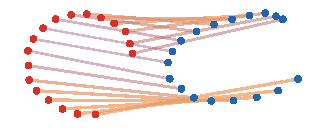
\includegraphics[width=.43\linewidth]{figures/gromov-nonisometric-distortion--correspondence.pdf} &
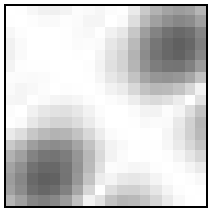
\includegraphics[width=.23\linewidth]{figures/gromov-nonisometric-distortion--distance-residual.pdf}
\\[-.1em]
\small hard correspondence $\sigma$ &
\small residual $|d_\X-d_\Y\circ\sigma|$
\end{tabular}
\caption{\emph{Local distortion in a mildly non-isometric GW match.} The left panel colors transport segments by the average residual induced by the displayed hard correspondence. The right panel shows the pairwise-distance residual matrix $|d_\X(x_i,x_{i'})-d_\Y(y_{\sigma(i)},y_{\sigma(i')})|$ in white-to-black scale, with darker entries marking larger local distortion. This matrix is the local contribution minimized by the discrete GW objective for the displayed correspondence.}
\index{distance residual}% strictindex
\index{distortion}% strictindex
\index{correspondence}% strictindex
\label{fig:gromov-nonisometric-distortion}
\end{figure}

We now record the profile lower bound used above as a useful initialization principle for the non-convex solver. The construction maps each point to its distance-profile distribution and then pushes forward the ambient measure, thereby producing a distribution over distributions. It is therefore a direct instance of the Wasserstein-over-Wasserstein geometry defined in~\eqref{eq-wow-distance} and developed in Section~\ref{sec-wasserstein-over-wasserstein}.
\index{profile lower bound}% strictindex

\begin{prop}[M\'emoli profile lower bound]\label{prop-memoli-gw-profile-lower-bound}
\index{Memoli profile@M\'emoli profile}% strictindex
	Let $\XX=(\X,\dist_\X,\alpha)$ and $\YY=(\Y,\dist_\Y,\beta)$ be compact metric-measure spaces and take $\De(u,v)=|u-v|$ in~\eqref{eq-gw-generic}, with the same exponent $p\geq1$. For each $x\in\X$ and $y\in\Y$, define the distance-profile measures on $\RR_+$ by
\index{metric-measure space}% strictindex
	\[
		\alpha_x\eqdef(\dist_\X(x,\cdot))_\sharp\alpha,
		\qquad
		\beta_y\eqdef(\dist_\Y(y,\cdot))_\sharp\beta.
	\]
	Let $\mathfrak D_\XX=(x\mapsto\alpha_x)_\sharp\alpha$ and $\mathfrak D_\YY=(y\mapsto\beta_y)_\sharp\beta$, which are probability measures on $\Pp_p(\RR_+)$. Then
\index{probability measure}% strictindex
	\[
		\mathbb W_p\bigl(\mathfrak D_\XX,\mathfrak D_\YY\bigr)
		\leq
		\GW(\XX,\YY).
	\]
	Here $\mathbb W_p$ is the Wasserstein-over-Wasserstein distance~\eqref{eq-wow-distance}: its ground space is $(\Pp_p(\RR_+),\Wass_p)$.
\index{ground cost}% strictindex
\index{Wasserstein!distance}% strictindex
\end{prop}
\begin{proof}
	Fix any $\pi\in\Couplings(\alpha,\beta)$. It induces a coupling $(x,y)\mapsto(\alpha_x,\beta_y)$ between $\mathfrak D_\XX$ and $\mathfrak D_\YY$, hence
	\[
		\mathbb W_p\bigl(\mathfrak D_\XX,\mathfrak D_\YY\bigr)^p
		\leq
		\int_{\X\times\Y}\Wass_p(\alpha_x,\beta_y)^p\,\d\pi(x,y).
	\]
	For fixed $(x,y)$, the map $(x',y')\mapsto(\dist_\X(x,x'),\dist_\Y(y,y'))$ pushes the same coupling $\pi$ to a coupling between $\alpha_x$ and $\beta_y$. Therefore
	\[
		\Wass_p(\alpha_x,\beta_y)^p
		\leq
		\int_{\X\times\Y}
		\abs{\dist_\X(x,x')-\dist_\Y(y,y')}^p
		\d\pi(x',y').
	\]
	Integrating in $(x,y)$ gives
	\[
		\mathbb W_p\bigl(\mathfrak D_\XX,\mathfrak D_\YY\bigr)^p
		\leq
		\int_{\X^2\times\Y^2}
		\abs{\dist_\X(x,x')-\dist_\Y(y,y')}^p
		\d\pi(x,y)\d\pi(x',y').
	\]
	Taking the infimum over $\pi$ and then the $p$-th root proves the claim.
\end{proof}

Figure~\ref{fig:gromov-memoli-distance-profiles} makes the two transport levels explicit on densely sampled silhouettes: sorting each distance row computes the one-dimensional profile costs exactly, then an outer assignment couples the resulting empirical profile laws.

\begin{figure}[ht]
\centering
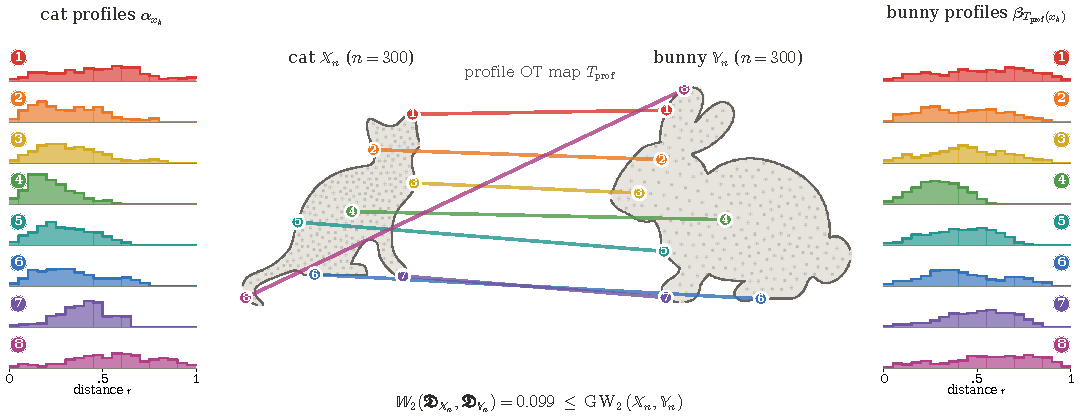
\includegraphics[width=.99\linewidth]{figures/gromov-memoli-distance-profiles/profiles.pdf}
\caption{\emph{M\'emoli distance profiles expose a computable lower bound for intrinsic GW comparison.} The cat and bunny silhouettes are each discretized by $300$ well-spread farthest-point samples and normalized to unit diameter. A second farthest-point pass selects eight representative cat anchors; their bunny partners are the exact images under the optimal equal-weight assignment with cost $C_{ij}=\Wass_2^2(\alpha_{x_i},\beta_{y_j})$. Matching colors identify each anchor pair, its transport segment and the two profile histograms in the side columns. The histograms use $20$ bins only for visualization: every entry of $C$ is computed without binning by sorting all $300$ distances in both profiles. The value displayed below is therefore the certified profile lower bound $\mathbb W_2(\mathfrak D_\XX,\mathfrak D_\YY)\leq\GW(\XX,\YY)$.}
\label{fig:gromov-memoli-distance-profiles}
\index{Memoli profile@M\'emoli profile}% strictindex
\index{distance profile}% strictindex
\index{Wasserstein-over-Wasserstein}% strictindex
\end{figure}

This lower bound is useful computationally because the profile cost matrix $\C_{ij}=\Wass_p(\alpha_{x_i},\beta_{y_j})^p$ is an ordinary OT cost between points. Solving this easier OT problem gives a geometry-aware initialization for the non-convex GW iterations below, before the full pairwise-distance distortion is optimized.

\paragraph{Relation with Wasserstein--Procrustes.}
\index{Wasserstein!Procrustes}% strictindex
\index{quotient Wasserstein distance}% strictindex
The profile lower bound is intrinsic. In Euclidean applications, it is naturally paired with an extrinsic upper certificate obtained by registering the two measures before applying the ordinary Wasserstein distance.
Proposition~\ref{prop-gw-procrustes-upper-certificate}, proved in the Wasserstein--Procrustes discussion of Section~\ref{sec-quotient-wasserstein-procrustes}, supplies exactly this certificate. The converse need not hold, because a small GW value may be achieved by an intrinsic correspondence that is not induced by any ambient rigid motion. Combining that proposition with Proposition~\ref{prop-memoli-gw-profile-lower-bound} gives the Euclidean sandwich
\index{Wasserstein!Procrustes}% strictindex
\begin{equation}\label{eq-gw-profile-procrustes-sandwich}
\mathbb W_p(\mathfrak D_\XX,\mathfrak D_\YY)
\leq
\GW(\XX,\YY)
\leq
2\,\Wass_{p,\mathrm E(d)}([\alpha],[\beta]),
\end{equation}
where $\XX=(\RR^d,\norm{\cdot},\alpha)$ and $\YY=(\RR^d,\norm{\cdot},\beta)$. The left term is intrinsic and inexpensive, while the right term is an extrinsic rigid-registration certificate.
\index{distortion}% strictindex
\index{cost!matrix}% strictindex
\index{Wasserstein!Procrustes}% strictindex

\paragraph{Entropic regularization and iterative solver.}
\index{entropic!regularization}% strictindex

For the common squared distortion $\De(u,v)^2=(u-v)^2$, one often seeks a stationary point of the entropic relaxation
\index{stationarity}% strictindex
\eql{\label{eq-gw-entropy}
	\umin{\P\in\CouplingsD(\a,\b)}
	\Ee_{\distD,\distD'}(\P)-\epsilon\HD(\P).
}
For symmetric distance matrices, define the half-gradient
\index{linear!linearization}% strictindex
\eql{\label{eq-gw-sinkh}
	\C(\P)
	\eqdef
	\distD^{\odot2}\a\,\ones_m^\top
	+
	\ones_n(\distD'^{\odot2}\b)^\top
	-
	2\distD\,\P\,\transp{\distD'},
	\qquad
	\nabla\Ee_{\distD,\distD'}(\P)=2\C(\P).
}
A standard fixed-point linearization~\cite{peyre2016gromov} computes
\[
	\P^{(k+1)}
	=
	\uargmin{\P\in\CouplingsD(\a,\b)}
	\dotp{\C(\P^{(k)})}{\P}-\frac{\epsilon}{2}\HD(\P).
\]
The factor $\epsilon/2$ is essential because~\eqref{eq-gw-sinkh} is one half of the gradient of the quadratic term. Each update is an ordinary entropic OT problem and can therefore be solved with Sinkhorn iterations. If the iterates converge to a positive fixed point, that point satisfies the first-order stationarity conditions of~\eqref{eq-gw-entropy}. The basic iteration is not a descent method in general and offers no global guarantee for this non-convex objective; line searches or proximal variants can be used when monotone decrease is required.
\index{Sinkhorn!iteration}% strictindex
\index{entropic!OT}% strictindex

\begin{alg}[Entropic Gromov--Wasserstein linearization]\label{alg:entropic-gromov-wasserstein}
\textbf{Input:} Symmetric metric matrices $\distD,\distD'$, weights $\a,\b$, regularization $\epsilon>0$, tolerance $\mathrm{tol}$, maximum iterations $L$.

\textbf{Output:} Approximate entropic GW coupling $\P\in\CouplingsD(\a,\b)$.

\textbf{Initialize:} Set $\P^{(0)}=\a\otimes\b$.

\textbf{For} $k=0,\ldots,L-1$ \textbf{do}:
\begin{algblock}
\(\C^{(k)} = \distD^{\odot2}\a\,\ones_m^\top + \ones_n(\distD'^{\odot2}\b)^\top - 2\distD\,\P^{(k)}\,\transp{\distD'}\).

\textbf{Solve} entropic OT subproblem:
\(\P^{(k+1)} = \uargmin{\P\in\CouplingsD(\a,\b)} \dotp{\P}{\C^{(k)}}-(\epsilon/2)\HD(\P)\).

\textbf{If} $\norm{\P^{(k+1)}-\P^{(k)}}_{\mathrm F}\leq\mathrm{tol}$ \textbf{then}:
\begin{algblock}
\textbf{Return} $\P^{(k+1)}$.
\end{algblock}
\end{algblock}
\algreturnskip
\textbf{Return} $\P^{(L)}$.
\end{alg}

\paragraph{Adding features.}
\index{feature cost}% strictindex
Fused Gromov--Wasserstein augments the structural term with a feature transport cost~\cite{vayer2019optimaltransportstructured}. In the discrete case, given a cross-feature cost $M\in\RR^{n\times m}$ and a parameter $\lambda\in[0,1]$, one minimizes
\index{Gromov-Wasserstein@Gromov--Wasserstein}% strictindex
\index{fused Gromov-Wasserstein}% strictindex
\[
	\operatorname{FGW}_{\lambda,p}((\a,\distD),(\b,\distD'))^p
	\eqdef
	\umin{\P\in\CouplingsD(\a,\b)}
	(1-\lambda)\sum_{i,j}M_{ij}\P_{ij}
	+\lambda
	\sum_{i,j,i',j'}\De(\distD_{ii'},\distD'_{jj'})^p\P_{ij}\P_{i'j'}.
\]
The first term compares node attributes in the usual OT sense, while the second compares the intrinsic geometry. The endpoints $\lambda=0$ and $\lambda=1$ recover feature-only OT and pure GW respectively; intermediate values trade attribute matching against structural matching. This is useful when the two spaces have both distances and features, and these two sources of information may disagree.

Figure~\ref{fig:fused-gromov-feature-geometry} isolates this tradeoff on a small graph pair by comparing feature-only, structure-only and fused correspondences.

\begin{figure}[ht]
\centering
\begin{tabular}{@{}ccc@{}}
\small feature-only OT &
\small fused GW &
\small pure GW \\[-.15em]
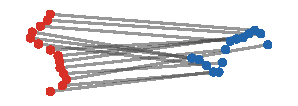
\includegraphics[width=.30\linewidth]{figures/fused-gromov-feature-geometry--feature-ot.pdf} &
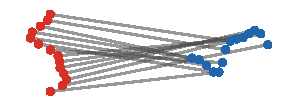
\includegraphics[width=.30\linewidth]{figures/fused-gromov-feature-geometry--fused-gw.pdf} &
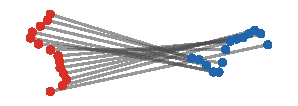
\includegraphics[width=.30\linewidth]{figures/fused-gromov-feature-geometry--pure-gw.pdf}
\end{tabular}
\caption{\emph{Feature information and intrinsic geometry in fused Gromov--Wasserstein.} Small inner disks encode binary node features. Feature-only OT follows the attributes even when this crosses the shape structure, pure GW follows the intrinsic ordering, and fused GW balances the feature term with the pairwise-distance distortion.}
\index{feature term}% strictindex
\index{node feature}% strictindex
\index{distortion}% strictindex
\index{fused Gromov-Wasserstein}% strictindex
\label{fig:fused-gromov-feature-geometry}
\end{figure}

\begin{example}[Application to multi-omics alignment]\label{ex-multi-omics-alignment}
\index{multi-omics}% strictindex
\index{single-cell genomics}% strictindex
	Multi-omics experiments can produce unmatched point clouds in different feature spaces, for instance RNA and ATAC profiles measured on different cells. If direct feature comparison is unavailable or incomplete, the relational term in GW preserves neighborhood structure; if partial cross-feature information exists, fused GW uses it through \(M_{ij}\). Unbalanced and co-optimal variants further allow the number and relative importance of cells or features to differ across modalities. The mathematical template is therefore precise: preserve within-modality geometry while learning a cross-modality coupling~\cite{TranJanatiCourtyFlamaryRedkoDemetciSingh2022UCOOT,RyuBunnePinelloRegevLopez2024LabeledGW,StanojevicLiGarmire2022MultiOmicsReview}.
\end{example}

\paragraph{Hausdorff and Gromov--Hausdorff viewpoints.}
\index{Hausdorff distance}% strictindex
\index{Gromov-Hausdorff distance}% strictindex

If $A,B$ are compact subsets of a common metric space $(\Z,\dist_\Z)$, their Hausdorff distance is
\[
	d_{\mathrm H}^{\Z}(A,B)
	=
	\max\left\{
		\sup_{a\in A}\inf_{b\in B}\dist_\Z(a,b),
		\sup_{b\in B}\inf_{a\in A}\dist_\Z(a,b)
	\right\}.
\]
The Gromov--Hausdorff distance removes the common ambient space by minimizing this quantity over all isometric embeddings into a third space:
\index{isometric embedding}% strictindex
\index{Hausdorff distance}% strictindex
\index{Gromov-Hausdorff distance}% strictindex
\[
	d_{\mathrm{GH}}(\X,\Y)
	=
	\inf_{\Z,\phi,\psi}
	d_{\mathrm H}^{\Z}(\phi(\X),\psi(\Y)).
\]
Equivalently, it is half the minimal distortion of a correspondence between $\X$ and $\Y$~\cite{gromov-2001,memoli-2007}. This is a worst-case set distance: every point must be matched with small distortion. Gromov--Wasserstein replaces correspondences by probability couplings and worst-case distortion by averaged distortion. It is therefore better adapted to noisy sampled shapes and weighted graphs, but it can ignore small sets of mass that would dominate the Hausdorff distance.
\index{distortion}% strictindex
\index{correspondence}% strictindex
\index{Gromov-Wasserstein@Gromov--Wasserstein}% strictindex
\index{Hausdorff distance}% strictindex

\section{Quantum Optimal Transport}
\index{quantum!OT}% strictindex
\label{sec-quantum-ot}

Quantum optimal transport replaces probability vectors by density matrices and scalar couplings by positive operators on a tensor product space. This is the right language when the transported objects are matrix-valued signals, covariance-like descriptors or quantum states, and it exposes a precise bridge between OT, non-commutative entropy and operator scaling. The finite-dimensional formulation below follows the semidefinite viewpoint developed in matrix-valued and quantum OT~\cite{Ning2014metrics,Chen2016,ChenGangbo17,2016-peyre-qot,caglioti2019quantum,chakrabarti2019quantum}.
\index{positive!operator}% strictindex
\index{quantum!OT}% strictindex
\index{operator scaling}% strictindex
\index{density!matrix}% strictindex

\paragraph{Finite-dimensional states and couplings.}
\index{quantum!coupling}% strictindex

The finite-dimensional case is the cleanest quantum analogue of the Kantorovich formulation. Probability vectors are replaced by positive semidefinite, trace-one matrices, and a coupling becomes a positive semidefinite operator on a tensor product whose partial traces prescribe the two marginals. This keeps the familiar ``joint object with fixed marginals'' geometry, while turning the transport problem into a semidefinite program.

\begin{defn}[Hermitian and density matrices]\label{def-hermitian-density-matrices}
\index{Hermitian matrix}% strictindex
	Let $\mathbb H_n$ be the real vector space of $n\times n$ Hermitian matrices,
	\[
		\mathbb H_n^+
		=
		\enscond{A\in\mathbb H_n}{A\succeq0},
		\qquad
		\mathbb H_n^{+,1}
		=
		\enscond{A\in\mathbb H_n^+}{\tr(A)=1}.
	\]
	Here $A\succeq0$ means that $A$ is positive semidefinite, namely $z^*Az\geq0$ for every $z\in\CC^n$, or equivalently that all eigenvalues of $A$ are nonnegative.
	Elements of $\mathbb H_n^{+,1}$ are density matrices.
\index{density!matrix}% strictindex
\end{defn}

For $A\in\mathbb H_n$ and $B\in\mathbb H_m$, the tensor product $A\otimes B$ is the linear operator determined by
\begin{equation}\label{eq-qot-tensor-product}
	(A\otimes B)(x\otimes y)=(Ax)\otimes(By),
	\qquad
	A\otimes B=[A_{i,k}B]_{i,k=1}^n,
	\qquad
	(A\otimes B)_{(i,j),(k,\ell)}=A_{i,k}B_{j,\ell}.
\end{equation}

\begin{defn}[Joint quantum states and partial traces]\label{def-joint-quantum-state}
\index{trace!partial}% strictindex
A joint quantum state between $\CC^n$ and $\CC^m$ is a density matrix $T\in\mathbb H_{nm}^{+,1}$ acting on $\CC^n\otimes\CC^m$. Its marginals are the partial traces $\operatorname{Tr}_B(T)\in\mathbb H_n^{+,1}$ and $\operatorname{Tr}_A(T)\in\mathbb H_m^{+,1}$ defined, for all $F\in\mathbb H_n$ and $G\in\mathbb H_m$, by
\begin{equation}\label{eq-qot-partial-traces}
	\tr(F\,\operatorname{Tr}_B T)=\tr((F\otimes\Id_m)T),
	\qquad
	\tr(G\,\operatorname{Tr}_A T)=\tr((\Id_n\otimes G)T),
\end{equation}
and they play the role of the two marginals of a classical coupling.
\end{defn}

In product bases $(e_i)_{i=1}^n$ and $(f_j)_{j=1}^m$, the operator $T$ can equivalently be viewed as the four-index tensor
\[
	T_{(i,j),(k,\ell)}
	=
	\langle e_i\otimes f_j,T(e_k\otimes f_\ell)\rangle.
\]
The full and partial traces then read
\begin{equation}\label{eq-qot-partial-traces-indices}
	\tr(T)=\sum_{i=1}^n\sum_{j=1}^m T_{(i,j),(i,j)},
	\qquad
	[\operatorname{Tr}_B T]_{i,k}=\sum_{j=1}^m T_{(i,j),(k,j)},
	\qquad
	[\operatorname{Tr}_A T]_{j,\ell}=\sum_{i=1}^n T_{(i,j),(i,\ell)}.
\end{equation}
In particular, $\tr(T)=\tr(\operatorname{Tr}_B T)=\tr(\operatorname{Tr}_A T)$. The feasible set below is never empty, since $A\otimes B$ has partial traces $A$ and $B$ whenever $A$ and $B$ are density matrices.

\begin{defn}[Finite-dimensional quantum OT]\label{def-finite-dimensional-qot}
\index{quantum!OT}% strictindex
	Let $A\in\mathbb H_n^{+,1}$, $B\in\mathbb H_m^{+,1}$ and let $C\in\mathbb H_{nm}$ be a Hermitian cost observable. The quantum OT value is the semidefinite program
\index{semidefinite program}% strictindex
\index{Hermitian matrix}% strictindex
\index{quantum!OT}% strictindex
	\begin{equation}\label{eq-qot-primal}
		\mathrm{QOT}_C(A,B)
		\eqdef
		\min_{T\in\mathbb H_{nm}^+}
		\enscond{\tr(CT)}{\operatorname{Tr}_B(T)=A,\ \operatorname{Tr}_A(T)=B}.
	\end{equation}
\end{defn}

\begin{example}[Classical diagonal case]\label{rem-qot-classical-diagonal-case}
	Suppose that $A$, $B$ and $C$ are diagonal in fixed product bases. Let $\Delta_A$ and $\Delta_B$ be the corresponding dephasing maps. For every feasible $T$, the matrix $\widetilde T=(\Delta_A\otimes\Delta_B)(T)$ is positive, has the same partial traces, and satisfies $\tr(C\widetilde T)=\tr(CT)$. Hence an optimal coupling may be chosen diagonal. Its diagonal entries form a nonnegative matrix with row sums given by $A$ and column sums given by $B$, so~\eqref{eq-qot-primal} reduces exactly to classical Kantorovich OT. The genuinely quantum feature is that non-commuting data may require off-diagonal coherences or entanglement.
\index{trace!partial constraint}% strictindex
\end{example}


\begin{prop}[Quantum Kantorovich duality]\label{prop-qot-duality}
\index{Kantorovich!duality}% strictindex
\index{quantum!Kantorovich duality}% strictindex
	For $A\in\mathbb H_n^{+,1}$ and $B\in\mathbb H_m^{+,1}$, the dual of~\eqref{eq-qot-primal} is
	\begin{equation}\label{eq-qot-dual}
		\mathrm{QOT}_C(A,B)
		=
		\sup_{F\in\mathbb H_n,\ G\in\mathbb H_m}
		\left\{
			\tr(FA)+\tr(GB)
			:\,
			F\otimes\Id_m+\Id_n\otimes G\preceq C
		\right\}.
	\end{equation}
	There is no duality gap. If $A$ and $B$ are positive definite, the supremum is attained. For singular marginals, the primal reduces to the tensor product of their supports; on this reduced space the corresponding dual maximum is attained, while the full-space formula above is always valid as a supremum.
\index{duality!strong}% strictindex
\index{Slater condition}% strictindex
\end{prop}

\begin{proof}
	Introduce Hermitian Lagrange multipliers $F$ and $G$ for the two marginal constraints. The Lagrangian is
\index{Hermitian matrix}% strictindex
\index{marginal!constraint}% strictindex
	\[
		\tr(CT)+\tr\!\left(F(A-\operatorname{Tr}_B T)\right)
		+\tr\!\left(G(B-\operatorname{Tr}_A T)\right)
		=
		\tr(FA)+\tr(GB)
		+\tr\!\left((C-F\otimes\Id_m-\Id_n\otimes G)T\right),
	\]
	where~\eqref{eq-qot-partial-traces} was used in the last equality. Minimizing over $T\succeq0$ gives a finite lower bound if and only if $C-F\otimes\Id_m-\Id_n\otimes G\succeq0$, in which case the infimum in $T$ is $0$. This gives the dual program. When $A,B\succ0$, the coupling $A\otimes B$ is strictly feasible, so Slater's theorem gives equality of primal and dual values and dual attainment.

	For singular marginals, let $P_A$ and $P_B$ be their support projections. If $T$ is feasible, then
	\[
		\tr\bigl(((\Id_n-P_A)\otimes\Id_m)T\bigr)
		=
		\tr((\Id_n-P_A)A)=0.
	\]
	Positivity implies that $T$ vanishes on $(\supp A)^\perp\otimes\CC^m$; the analogous argument for $B$ yields
	\[
		T=(P_A\otimes P_B)T(P_A\otimes P_B).
	\]
	Thus the primal is exactly the problem obtained by compressing $A$, $B$ and $C$ to $\supp A\otimes\supp B$. The reduced marginals are positive definite, so Slater applies there. Equivalently, the unreduced dual values approach the reduced maximum after assigning sufficiently negative potentials on the orthogonal complements. This proves the stated supremum formula without a gap.
\index{Slater condition}% strictindex
\index{dual!attainment}% strictindex
\index{trace!partial}% strictindex
\end{proof}

The dual potentials have the usual scalar gauge freedom: replacing $(F,G)$ by $(F+t\Id_n,G-t\Id_m)$ leaves both the constraint and the value unchanged because $\tr(A)=\tr(B)=1$.
\index{dual!potential}% strictindex

\paragraph{Entropic regularization and Bregman iterations.}
\index{entropic!regularization}% strictindex
\index{Bregman!iteration}% strictindex
As in scalar OT, one obtains a smoother problem by adding the convex quantum entropy functional associated with the matrix logarithm.

\begin{defn}[von Neumann quantum entropy]\label{def-von-neumann-quantum-entropy}
\index{von Neumann entropy}% strictindex
	For a density matrix or positive semidefinite matrix $T$, the shifted von Neumann entropy functional used here is
\index{density!matrix}% strictindex
	\[
		H(T)=\tr\!\left(T(\log T-\Id)\right),
		\qquad
		\nabla H(T)=\log T,
	\]
	with the convention $0\log0=0$ on eigenvalues. This is the convex negative quantum entropy; on trace-one states it differs from the physical entropy $-\tr(T\log T)$ by a sign and an additive constant.
\end{defn}
For $\epsilon>0$ define
\begin{equation}\label{eq-qot-entropic-primal}
	\mathrm{QOT}_C^\epsilon(A,B)
	=
	\min_{T\succeq0}
	\left\{
		\tr(CT)+\epsilon H(T)
		:\,
		\operatorname{Tr}_B(T)=A,
		\operatorname{Tr}_A(T)=B
	\right\}.
\end{equation}
This is the non-commutative analogue of entropic OT~\cite{2016-peyre-qot,chakrabarti2019quantum}: the Shannon entropy of a coupling is replaced by the trace entropy of a density matrix.
\index{trace!entropy}% strictindex
\index{entropic!OT}% strictindex
\index{Shannon entropy}% strictindex
\index{density!matrix}% strictindex

\begin{prop}[Entropic quantum OT duality]\label{prop-qot-entropic-duality}
\index{quantum!OT}% strictindex
\index{quantum!OT duality}% strictindex
	Assume $A\succ0$, $B\succ0$ and $\epsilon>0$. Then~\eqref{eq-qot-entropic-primal} has a unique positive minimizer. Its dual is
	\begin{equation}\label{eq-qot-entropic-dual}
		\mathrm{QOT}_C^\epsilon(A,B)
		=
		\max_{F\in\mathbb H_n,\ G\in\mathbb H_m}
		\left\{
			\tr(FA)+\tr(GB)
			-\epsilon\,
			\tr\exp\!\left(\frac{F\otimes\Id_m+\Id_n\otimes G-C}{\epsilon}\right)
		\right\}.
	\end{equation}
	At optimality, primal and dual variables are linked by the Gibbs formula
\index{Gibbs!formula}% strictindex
	\begin{equation}\label{eq-qot-gibbs-coupling}
		T_e(F,G)
		=
		\exp\!\left(\frac{F\otimes\Id_m+\Id_n\otimes G-C}{\epsilon}\right),
	\end{equation}
	with $\operatorname{Tr}_B(T_e)=A$ and $\operatorname{Tr}_A(T_e)=B$.
\end{prop}

\begin{proof}
	The feasible set is compact and nonempty, and it contains the positive definite point $A\otimes B$. The trace entropy is strictly convex on positive semidefinite matrices, hence the regularized primal has a unique minimizer. This minimizer is positive definite: if it had a non-trivial kernel, moving toward $A\otimes B$ would have entropy directional derivative $-\infty$ at the boundary while changing the linear cost only at finite rate. Slater's condition justifies the Lagrange dual computation. The Fenchel identity
\index{trace!entropy}% strictindex
\index{Slater condition}% strictindex
\index{positive!semidefinite matrix}% strictindex
	\[
		\sup_{T\succeq0}\ \tr(YT)-\epsilon H(T)
		=
		\epsilon\,\tr\exp(Y/\epsilon)
	\]
	is the matrix analogue of the scalar exponential conjugacy. Applying it to the Lagrangian of~\eqref{eq-qot-entropic-primal}, with
	$Y=F\otimes\Id_m+\Id_n\otimes G-C$, gives~\eqref{eq-qot-entropic-dual}. The stationarity condition of this Fenchel identity gives~\eqref{eq-qot-gibbs-coupling}; differentiating the dual objective with respect to $F$ and $G$ yields the two marginal equations.
\index{stationarity}% strictindex
\index{Gibbs!coupling}% strictindex
\end{proof}

Writing $K=\exp(-C/\epsilon)$, the objective in~\eqref{eq-qot-entropic-primal} differs by a constant from $\epsilon$ times the quantum KL divergence
\[
	D_H(T|K)
	=
	\tr\!\left(T(\log T-\log K)-T+K\right).
\]
The exact quantum analogue of Sinkhorn is an implicit alternating Bregman projection scheme onto the affine marginal sets
\index{Bregman!projection}% strictindex
\[
	\mathcal M_A=\{T\succeq0:\operatorname{Tr}_B(T)=A\},
	\qquad
	\mathcal M_B=\{T\succeq0:\operatorname{Tr}_A(T)=B\}.
\]

\begin{prop}[Exact Bregman projections]\label{prop-qot-bregman-projections}
	Assume $A,B\succ0$ and let $K=\exp(-C/\epsilon)$. The minimizer of~\eqref{eq-qot-entropic-primal} is equivalently the minimizer of $D_H(T|K)$ over $\mathcal M_A\cap\mathcal M_B$. Moreover, if a current positive definite matrix has Gibbs form $T_e(F,G)$, then its Bregman projection onto $\mathcal M_A$ has the form $T_e(F^+,G)$, where $F^+$ is chosen so that $\operatorname{Tr}_B T_e(F^+,G)=A$. The projection onto $\mathcal M_B$ is analogous. Thus, when each one-block marginal equation is solved exactly, alternating Bregman projections are equivalent to alternating block maximization of the dual~\eqref{eq-qot-entropic-dual}.
\end{prop}

\begin{proof}
	Since $\log K=-C/\epsilon$, the identity
	\[
		\tr(CT)+\epsilon H(T)
		=
		\epsilon D_H(T|K)-\epsilon\tr(K)
	\]
	holds, so the primal minimizer is the constrained Bregman projection of $K$ up to an additive constant. For the projection of a positive definite matrix $S$ onto $\mathcal M_A$, the affine set contains the positive definite point $A\otimes\Id_m/m$; the entropy derivative $\log T-\log S$ is singular at the boundary, so the projection lies in the interior of the positive cone. Its Lagrangian first variation is
\index{first variation}% strictindex
\index{Bregman!projection}% strictindex
\index{positive!cone}% strictindex
	\[
		\log T-\log S-\Lambda\otimes\Id_m=0
	\]
	for a Hermitian multiplier $\Lambda$. Hence $T=\exp(\log S+\Lambda\otimes\Id_m)$. If $S=T_e(F,G)$, this is again of the form $T_e(F+\epsilon\Lambda,G)$. The multiplier is fixed by the marginal equation $\operatorname{Tr}_B(T)=A$. The same argument applies to $\mathcal M_B$. Finally, the first-order optimality condition for maximizing~\eqref{eq-qot-entropic-dual} over one block is exactly the corresponding marginal equation, so the Bregman and block-dual views coincide.
\index{Hermitian matrix}% strictindex
\index{optimality!first-order}% strictindex
\end{proof}

In the diagonal case this proposition gives the usual multiplicative Sinkhorn updates. In the non-commutative case, however, the exact block equations
\index{Sinkhorn!update}% strictindex
\[
	\operatorname{Tr}_B T_e(F,G)=A,
	\qquad
	\operatorname{Tr}_A T_e(F,G)=B
\]
do not admit scalar division formulas, because the exponential of $F\otimes\Id_m+\Id_n\otimes G-C$ cannot be separated unless the local potential $F\otimes\Id_m+\Id_n\otimes G$ commutes with the cost $C$.
When all matrices are diagonal in the same basis, commutativity restores the scalar form $T_e=\diag(u)K\diag(v)$ and the marginal equations reduce to the usual Sinkhorn divisions.

Algorithm~\ref{alg:quantum-exact-bregman} records this exact but implicit non-commutative analogue of Sinkhorn.

\begin{alg}[Exact quantum Bregman projections]\label{alg:quantum-exact-bregman}
\index{Bregman!projection}% strictindex
\index{quantum!Bregman projection}% strictindex
\textbf{Input:} Positive definite density matrices $A,B$, cost $C$, regularization $\epsilon>0$, tolerance $\mathrm{tol}$, maximum iterations $L$.

\textbf{Output:} Approximate quantum entropic coupling $T$ and its partial-trace residual.

\textbf{Initialize:} Set Hermitian potentials $F^{(0)}=0$ and $G^{(0)}=0$.

\textbf{For} $k=0,\ldots,L-1$ \textbf{do}:
\begin{algblock}
\(T^{(k)}= T_e(F^{(k)},G^{(k)}) = \exp\!\left( \frac{F^{(k)}\otimes\Id_m+\Id_n\otimes G^{(k)}-C}{\epsilon} \right)\).

\textbf{Solve} $A$-projection equation:
\(\operatorname{Tr}_B T_e(F^+,G^{(k)})=A\).

\textbf{Set} $F^{(k+1)}=F^+$.

\textbf{Solve} $B$-projection equation:
\(\operatorname{Tr}_A T_e(F^{(k+1)},G^+)=B\).

\textbf{Set} $G^{(k+1)}=G^+$.

\textbf{If} both partial-trace residuals are at most $\mathrm{tol}$ \textbf{then}:
\begin{algblock}
\textbf{Return} $T_e(F^{(k+1)},G^{(k+1)})$.
\end{algblock}
\end{algblock}
\algreturnskip
\textbf{Return} $T_e(F^{(L)},G^{(L)})$ and its residual.
\end{alg}

\paragraph{Gurvits scaling and quantum Sinkhorn.}
\index{Gurvits scaling}% strictindex
\index{quantum!Sinkhorn}% strictindex
The exact Bregman scheme above has a major computational obstruction: unlike classical marginal rescaling, projection onto either non-commutative marginal constraint requires solving a nonlinear matrix equation and has no closed form in general. Gurvits scaling instead provides an explicit fixed-point construction of a feasible quantum coupling, used as a surrogate for entropic QOT. Its iterates do not minimize the entropic QOT objective and, outside special commuting settings, do not generally arise as block minimizations of a global energy. In the diagonal case, however, the construction coincides with classical Sinkhorn, hence recovers its variational interpretation.

The algorithm often called quantum Sinkhorn comes from the operator-scaling literature of Gurvits and subsequent developments~\cite{gurvits2003classical,gurvits2004classical,georgiou2015positive,garg2018recent}. It replaces the true Gibbs coupling~\eqref{eq-qot-gibbs-coupling} by the symmetric factorization
\index{operator scaling}% strictindex
\index{Gibbs!coupling}% strictindex
\begin{equation}\label{eq-qot-symmetric-scaling}
	T_s(F,G)
	=
	\exp\!\left(\frac{Z}{2\epsilon}\right)\exp(-C/\epsilon)\exp\!\left(\frac{Z}{2\epsilon}\right)
	=
	(U\otimes V)K(U\otimes V),
	\qquad
	Z=F\otimes\Id_m+\Id_n\otimes G,
\end{equation}
where $U=\exp(F/(2\epsilon))$, $V=\exp(G/(2\epsilon))$ and $K=\exp(-C/\epsilon)$. For two matrices $M,N$, their commutator is $[M,N]\eqdef MN-NM$. Thus $[Z,C]=0$ means that $Z$ and $C$ commute; in this case $T_s(F,G)=T_e(F,G)$, whereas otherwise $T_s$ is a Strang-type symmetric surrogate.
\index{Strang splitting}% strictindex
\index{commutator}% strictindex

To make the Choi identification unambiguous, use the product bases fixed above and associate with $K$ the positive linear map $\mathcal K:\mathbb H_m\to\mathbb H_n$ and its Hilbert--Schmidt adjoint $\mathcal K^\star:\mathbb H_n\to\mathbb H_m$ through
\index{Choi matrix}% strictindex
\index{operator scaling}% strictindex
\index{scaling!form}% strictindex
\begin{equation}\label{eq-qot-choi-map}
	\mathcal K(X)
	\eqdef
	\operatorname{Tr}_B\!\bigl(K(\Id_n\otimes X)\bigr),
	\qquad
	\mathcal K^\star(Y)
	\eqdef
	\operatorname{Tr}_A\!\bigl(K(Y\otimes\Id_m)\bigr).
\end{equation}
Equivalently,
\[
	[\mathcal K(X)]_{i,k}
	=
	\sum_{j,\ell}K_{(i,j),(k,\ell)}X_{\ell,j},
	\qquad
	[\mathcal K^\star(Y)]_{j,\ell}
	=
	\sum_{i,k}K_{(i,j),(k,\ell)}Y_{k,i}.
\]
The adjoint relation is $\tr(Y\mathcal K(X))=\tr(\mathcal K^\star(Y)X)$. In the standard Choi convention, the completely positive map with Choi matrix $K$ is $X\mapsto\mathcal K(X^\top)$; the convention~\eqref{eq-qot-choi-map} merely places this basis-dependent transpose in the Choi identification rather than in the marginal equations. With this convention, the marginal equations for the symmetric coupling are exactly
\[
	U\,\mathcal K(V^2)\,U=A,
	\qquad
	V\,\mathcal K^\star(U^2)\,V=B.
\]
They can be enforced by the explicit congruence normalizations
\index{congruence normalization}% strictindex
\begin{equation}\label{eq-qot-gurvits-updates}
\begin{aligned}
	R_V&=\mathcal K(V^2),
	&
	U&\leftarrow
	R_V^{-1/2}\bigl(R_V^{1/2} A R_V^{1/2}\bigr)^{1/2}R_V^{-1/2},
	\\
	S_U&=\mathcal K^\star(U^2),
	&
	V&\leftarrow
	S_U^{-1/2}\bigl(S_U^{1/2} B S_U^{1/2}\bigr)^{1/2}S_U^{-1/2}.
\end{aligned}
\end{equation}
\begin{alg}[Gurvits/operator scaling for quantum Sinkhorn]\label{alg:quantum-gurvits-scaling}
\index{operator scaling}% strictindex
\textbf{Input:} Positive definite marginals $A,B$, positive definite kernel operator $K$, maps $\mathcal K,\mathcal K^\star$, tolerance $\mathrm{tol}$, maximum iterations $L$.

\textbf{Output:} Symmetrically scaled coupling $T_s$ with approximate prescribed marginals.

\textbf{Initialize:} Set $U=\Id_n$ and $V=\Id_m$.

\textbf{Set} residual \(r=+\infty\) and counter $k=0$.

\textbf{While} \(r>\mathrm{tol}\) and $k<L$ \textbf{do}:
\begin{algblock}
\(R_V=\mathcal K(V^2), \qquad U\leftarrow R_V^{-1/2}\bigl(R_V^{1/2} A R_V^{1/2}\bigr)^{1/2}R_V^{-1/2}\).

\(S_U=\mathcal K^\star(U^2), \qquad V\leftarrow S_U^{-1/2}\bigl(S_U^{1/2} B S_U^{1/2}\bigr)^{1/2}S_U^{-1/2}\).

\textbf{Set} \(T_s=(U\otimes V)K(U\otimes V)\) and \(r\) to the maximum of its two operator-marginal residuals against $A$ and $B$.

\textbf{Set} $k\leftarrow k+1$.
\end{algblock}
\algreturnskip
\textbf{Return} \(T_s\).
\end{alg}
These inverse square roots are well-defined when $K\succ0$ and $U,V,A,B\succ0$. Under the standard strict-positivity and scalability hypotheses, the alternating normalizations converge to the prescribed marginals~\cite{georgiou2015positive,garg2018recent}; the finite algorithm returns once the residual is below tolerance or the iteration budget is exhausted. This is Gurvits/operator scaling with prescribed targets. When all matrices are diagonal it reduces to classical Sinkhorn scaling, and when the targets are proportional to identities it matches the usual bistochastic operator-scaling normalization, up to the conventional trace normalization.
\index{Gurvits scaling}% strictindex
\index{inverse square root}% strictindex
\index{Sinkhorn!scaling}% strictindex
\index{operator scaling}% strictindex


\begin{rem}[Gurvits scaling is not the exact Bregman scheme]
	It is important not to identify~\eqref{eq-qot-gurvits-updates} with the exact Bregman scheme for~\eqref{eq-qot-entropic-primal}. The exact Bregman step would enforce the marginals of $T_e(F,G)=\exp((Z-C)/\epsilon)$ and would be a block maximization of the true concave dual~\eqref{eq-qot-entropic-dual}. Gurvits scaling instead enforces the marginals of the surrogate
\[
	T_s=
	\exp\!\left(\frac{Z}{2\epsilon}\right)
	\exp(-C/\epsilon)
	\exp\!\left(\frac{Z}{2\epsilon}\right).
\]
	The two coincide in the commuting/diagonal regime, but in general the Baker--Campbell--Hausdorff commutator terms do not vanish. The Gurvits iteration should therefore be understood as a tractable symmetric operator-scaling approximation to entropic Q--OT, not as the literal alternating KL projection algorithm or, in general, as block minimization of an underlying energy.
\index{Gurvits scaling}% strictindex
\index{commutator}% strictindex
\index{Baker-Campbell-Hausdorff formula}% strictindex
\index{operator scaling}% strictindex
\index{KL!projection}% strictindex
\end{rem}

\begin{rem}[Operator-valued couplings]
\index{operator-valued coupling}% strictindex
	The same definitions extend formally from matrices to separable Hilbert spaces by replacing density matrices with positive trace-class operators of trace one, observables with bounded self-adjoint operators and~\eqref{eq-qot-partial-traces} with partial traces defined by duality against local bounded observables. If $\Pi(A,B)$ denotes positive trace-class operators with partial traces $A$ and $B$, a bounded cost observable $C$ gives the problem $\inf_{T\in\Pi(A,B)}\Tr(CT)$. For unbounded positive costs one must define the energy through the quadratic form or spectral truncations, and in the entropic case one must ensure that the Gibbs operator $\exp(-C/\epsilon)$ is trace class and that the partial traces of the candidate coupling are well-defined. The matrix formulas above are therefore the clean finite-dimensional core; the operator version adds domain and compactness assumptions rather than a different algebraic structure.
\index{density!matrix}% strictindex
\index{trace-class operator}% strictindex
\index{trace!partial}% strictindex
\end{rem}

Vector, metric-measure and quantum transport thus extend the same coupling principle in three different directions: richer fibers, unknown cross-space correspondences and non-commutative joint states. The resulting feasible sets and algorithms differ substantially, but marginal constraints, convex duality and entropy regularization remain the common organizing mechanisms.
